\documentclass[fr]{../../../../../../eplexam}

\usepackage{../../../mmc-MECA1901-exam}

\hypertitle{MMC}{5}{MECA}{1901}{2017}{Janvier}
{Martin Braquet \and Etudiants BAC 3 (2016-2017)}
{Philippe Chatelain et Issam Doghri}

\section{Théorie}
\subsection{}
Soit a un tenseur d'ordre 2 non symétrique. On a les relations suivantes : $a:a$ et $a:1$. Développer avec la notation indicielle (et utiliser la notation d'Einstein). Sont-ils invariants sous les transformations tensorielles ?
\subsection{}
On a une fibre matérielle $\mathbf{dX}$ qui se déforme en $\mathbf{dx}$. Soit $\mathbf{B}=\mathbf{F}^T \cdot \mathbf{F}$, avec $\mathbf{F}$ le tenseur usuel du cours. Ecrire $$\frac{1}{2} \left(1 - \left(\frac{|\mathbf{dX}|}{|\mathbf{dx}|} \right)^2 \right)$$ uniquement en fonction de $\mathbf{B}$.

On voit apparaître quel tenseur?  Dans quelle configuration est-il défini?
\subsection{}
A partir de la forme globale de la conservation de la masse, montrez comment on arrive à $$ \frac{\partial \rho}{\partial t} + \mathbf{\nabla} \cdot (\rho \mathbf{v}) = 0 $$
Citez bien les théorèmes utilisé à chaque ligne.
\subsection{}
Pourquoi peut-on dire que $h(\hat{\mathbf{n}})=-\mathbf{q}\cdot \hat{\mathbf{n}}$ ?

A partir de quelle forme géométrique ou relation établit-on cette relation? 
Donnez un exemple de loi de constitution impliquant le flux de chaleur $\mathbf{q}$. Expliquez ensuite pourquoi cette loi est admissible.

\section{}
Un point matériel subit la transformation décrite ci dessous quand $t>0$ :
\begin{equation}
x_1= X_1+ \gamma X_2, \quad  x_2=X_2, \quad x_3=X_3
\end{equation}
Le tenseur de contraintes est donné par: 
\[
\bm{\sigma}=gJ^{-5/3}\mathrm{dev}(\mathbf{B})+h(J-1)\mathbf{I},
\]
sachant que $\mathbf{B}=\mathbf{F}^T \cdot \mathbf{F}$, que $g(t)$, $J=det(F)$ et $\gamma(t)>0$.

\begin{enumerate}
	\item Calculer $\bm{F}$.
	\item Calculer $\bm{\sigma}, \bm{B}$ et $J$ et commenter.
	\item Calculer les vecteurs de contraintes associées à des facettes ayant des normales $\Base{1}$, $\Base{2}$, $\Base{3}$. Représenter graphiquement. Commenter.
	\item Calculer les contraintes principales et les donner dans l'ordre décroissant
	\item Dessiner les cercles de Mohr et déterminer la contrainte de cisaillement maximale.
\end{enumerate}
	On considère maintenant des déformations infinitésimales, $ \bm{\epsilon} $ est le tenseur des déformations infinitésimales. A partir de maintenant, on n'applique plus les simplifications apportées par les équations des $x_i$.
\begin{enumerate}
	\setcounter{enumi}{5}
	\item Donner $\bm{B}$ et $J$ en fonction de $\bm{\epsilon} $ uniquement.
	\item Donner $\bm{\sigma} $ en fonction de $\bm{\epsilon} $, $g$ et $ h $, comparer avec l'équation (constitutive) du solide élastique isotrope.
	
	\item On suppose que $\gamma \ll 1$. Calculer $\bm{\sigma}$ (avec l'éq. 1). Commenter.
	
\end{enumerate}

\section{Exercice}

Même question que Q2 mineure janvier 2014 avec deux questions supplémentaires:

\begin{figure}[h!]
	\centering
	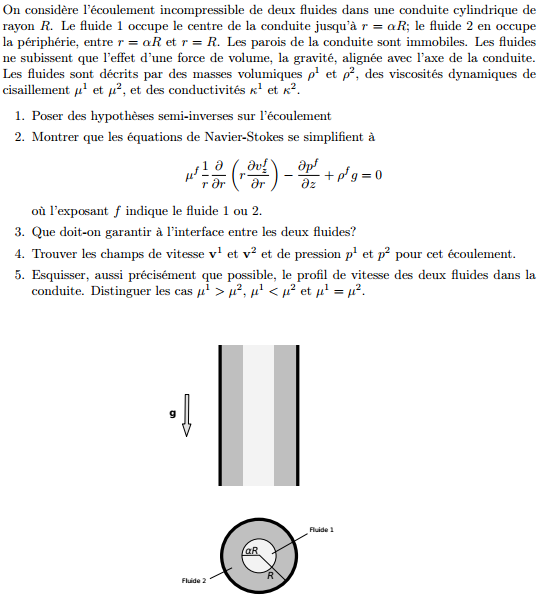
\includegraphics[scale=1]{Q2_MMC.png}
	\label{fig:my_label}
\end{figure}

\begin{enumerate}
	\setcounter{enumi}{5}
	\item Vérifier la conservation de la quantité de mouvement sur un volume de contrôle pour le fluide intérieur.
	\item Bonus : Vérifier la conservation de l'énergie sur un volume de contrôle pour le fluide intérieur.
\end{enumerate}

\end{document}
